%%
%% This is file `sample-sigconf.tex',
%% generated with the docstrip utility.
%%
%% The original source files were:
%%
%% samples.dtx  (with options: `sigconf')
%% 
%% IMPORTANT NOTICE:
%% 
%% For the copyright see the source file.
%% 
%% Any modified versions of this file must be renamed
%% with new filenames distinct from sample-sigconf.tex.
%% 
%% For distribution of the original source see the terms
%% for copying and modification in the file samples.dtx.
%% 
%% This generated file may be distributed as long as the
%% original source files, as listed above, are part of the
%% same distribution. (The sources need not necessarily be
%% in the same archive or directory.)
%%
%%
%% Commands for TeXCount
%TC:macro \cite [option:text,text]
%TC:macro \citep [option:text,text]
%TC:macro \citet [option:text,text]
%TC:envir table 0 1
%TC:envir table* 0 1
%TC:envir tabular [ignore] word
%TC:envir displaymath 0 word
%TC:envir math 0 word
%TC:envir comment 0 0
%%
%%
%% The first command in your LaTeX source must be the \documentclass command.
\documentclass[sigconf]{acmart}

%%
%% \BibTeX command to typeset BibTeX logo in the docs
\AtBeginDocument{%
  \providecommand\BibTeX{{%
    Bib\TeX}}}

%% Rights management information.  This information is sent to you
%% when you complete the rights form.  These commands have SAMPLE
%% values in them; it is your responsibility as an author to replace
%% the commands and values with those provided to you when you
%% complete the rights form.
\setcopyright{acmcopyright}
\copyrightyear{2022}
\acmYear{2022}
\acmDOI{XXXXXXX.XXXXXXX}

%% These commands are for a PROCEEDINGS abstract or paper.
\acmConference[Conference acronym 'XX]{Make sure to enter the correct
  conference title from your rights confirmation emai}{June 03--05,
  2022}{Austin, TX}
\acmPrice{15.00}
\acmISBN{978-1-4503-XXXX-X/18/06}


%%
%% Submission ID.
%% Use this when submitting an article to a sponsored event. You'll
%% receive a unique submission ID from the organizers
%% of the event, and this ID should be used as the parameter to this command.
%%\acmSubmissionID{123-A56-BU3}

%%
%% For managing citations, it is recommended to use bibliography
%% files in BibTeX format.
%%
%% You can then either use BibTeX with the ACM-Reference-Format style,
%% or BibLaTeX with the acmnumeric or acmauthoryear sytles, that include
%% support for advanced citation of software artefact from the
%% biblatex-software package, also separately available on CTAN.
%%
%% Look at the sample-*-biblatex.tex files for templates showcasing
%% the biblatex styles.
%%

%%
%% The majority of ACM publications use numbered citations and
%% references.  The command \citestyle{authoryear} switches to the
%% "author year" style.
%%
%% If you are preparing content for an event
%% sponsored by ACM SIGGRAPH, you must use the "author year" style of
%% citations and references.
%% Uncommenting
%% the next command will enable that style.
%%\citestyle{acmauthoryear}

%%
%% end of the preamble, start of the body of the document source.
\begin{document}

%%
%% The "title" command has an optional parameter,
%% allowing the author to define a "short title" to be used in page headers.
\title{What's in a Domain? Anaylsis of URL Features}

%%
%% The "author" command and its associated commands are used to define
%% the authors and their affiliations.
%% Of note is the shared affiliation of the first two authors, and the
%% "authornote" and "authornotemark" commands
%% used to denote shared contribution to the research.
\author{John Hawkins}
\email{john.hawkins@Getting-Data-Science-Done.com}
\orcid{1234-5678-9012}
\affiliation{%
  \institution{Getting-Data-Science-Done.com}
  \city{Sydney}
  \state{NSW}
  \country{Australia}
  \postcode{2000}
}

\renewcommand{\shortauthors}{Hawkins}

\begin{abstract}
Many data science problems require processing log data derived from web pages, apis or other
internet traffic sources. URLs are one of the few ubiquitous data fields that describe
internet activity, hence they require effective processing for a wide variety of machine 
learning applications. While URLs are structurally rich, they are not subject
to universal principles of construction making fetaure engineering for internet data an ongoing challenge.

In this research we outline the key categories of information structure in domains and URLs.
We share an open source implementation of these ideas and demonstrate their utility across a range of 
internet traffic machine learning problems. Python package available at https://pypi.org/project/url2features
\end{abstract}

%%
%% The code below is generated by the tool at http://dl.acm.org/ccs.cfm.
%% Please copy and paste the code instead of the example below.
%%

\begin{CCSXML}
<ccs2012>
<concept>
<concept_id>10002951.10003260.10003261</concept_id>
<concept_desc>Information systems~Web searching and information discovery</concept_desc>
<concept_significance>500</concept_significance>
</concept>
<concept>
<concept_id>10002951.10003260.10003277.10003280</concept_id>
<concept_desc>Information systems~Web log analysis</concept_desc>
<concept_significance>500</concept_significance>
</concept>
<concept>
<concept_id>10010147.10010257</concept_id>
<concept_desc>Computing methodologies~Machine learning</concept_desc>
<concept_significance>500</concept_significance>
</concept>
</ccs2012>
\end{CCSXML}

\ccsdesc[500]{Information systems~Web searching and information discovery}
\ccsdesc[500]{Information systems~Web log analysis}
\ccsdesc[500]{Computing methodologies~Machine learning}

\keywords{URL Features, Document Classification, Machine Learning, Semantic Web}

\maketitle

\section{Introduction}

The Uniform Resource Locator (URL) is a ubiquitous element the digital world. 
We use them to advertise and locate businesses, to retrieve news and media and 
to interact with other people across a broad of social applications.
Processing URLs is key component of many tasks that involve
analysing internet data. In many applications the URL is the central piece of 
information available because the demands of the task require immediate analysis.
In applications like malicious wesite detection the URL needs to be processed with
in a rapid and efficient manner to provide utility\cite{Ma2009b}.
Common use cases for URL centered analysis include security analysis of potenital phishing 
attacks\cite{Basnet2014,Mamun2016,Vazhayil2018}, and identification of pages 
that host malware or viruses \cite{Canali2011,Mamun2016}.
There are also applications to online advertising
including anticipation of conversions \cite{Qiu2020}, contextual analysis of
the content\cite{Kan2005,Baykan2009,Meshkizadeh2010} or language\cite{Baykan2013} of webpages. 

The URL is made up of multiple elements, but at its core is the domain. The domain
contains internal information about both its intended purpose, legitimacy and likely
origin. It is also a source of additional information through requests to Domain Name
Servers (DNS) to understand both its history and place within the network topology.

Common feature engineering strategies exploit these potential sources of information
in ways that are appropriate for a given task. However, while there are wide variety
of approaches that inconsistently applied, there has not yet been a study that evaluates
the overall effectiveness of different strategies across a range of applications.

In this work we describe an ontology of URL fetaures that relates to underlying origin
and purpose. We then present an open source package for generating features within these
ontologocal classes and apply them to a variety of tasks. We present our results as a
cross-task evaluation of URL features.  
 
A large amount of recent work on machine learning based on URLs has focused on deep learning approaches that
learn an embedding representation of the content of the URL. Once of the explicit reasons 
for this approach is the potential for sensitivity to the sequential structure of the URL.
\cite{Le2018}

Deep learning approaches include the use of convolutional layers to learn word and character 
embedings \cite{Le2018},

\cite{Ayes2019}
\cite{Li2020}
\cite{Basnet2012}
\cite{Basnet2014}
\cite{Tupsamudre2019}
\cite{Baykan2009}
\cite{Kan2005}
\cite{Hernandez2012}
\cite{Chung2010}
\cite{Qiu2020}
\cite{Xu2021}
\cite{Rhea2022}
\cite{Ma2009}
\cite{Verma2017}
\cite{Sountharrajan2020}
\cite{Murthy2022}

Classify Web pages based on URLs from the 4 Universities WebKB dataset. Comparing features derived from segmentation
of the URL to features derived from either link anchor text or the web page document itself \cite{Kan2004}.

Common approaches to feature engineering on URLs include string patterns and regular expressions to
identify key sequences and lexical properties \cite{Kan2004,Mamun2016}, 
creation of lookup tables or likelihood scores based on key sequences
\cite{Meshkizadeh2010}, n-gram or bag of words models \cite{Baykan2009}, 
the generation of task specific embedding vectors\cite{Le2018,Qiu2020} and the
usage of domain name servers or registrars for ancillary information about the domain registration \cite{Canali2011}. 
Some authors have 
emphasized that URLs are sequences of characters and require feature extraction methods that respect 
this sequential nature\cite{Le2018,Vazhayil2018}. They have naturally turned to developing neural network approaches
based on convolutional or recurrent layers for learning these sequential structures.
However, the ordering of key features within URLs is predominantly fixed as shown in Figure \ref{fig:url_structure}.
The core elements of URL structure occur at fixed positions within the sequence, in contrast to human language
sequences which are built from flexible grammars that allow variable positioning of most key elements.

\begin{figure*}
\centering
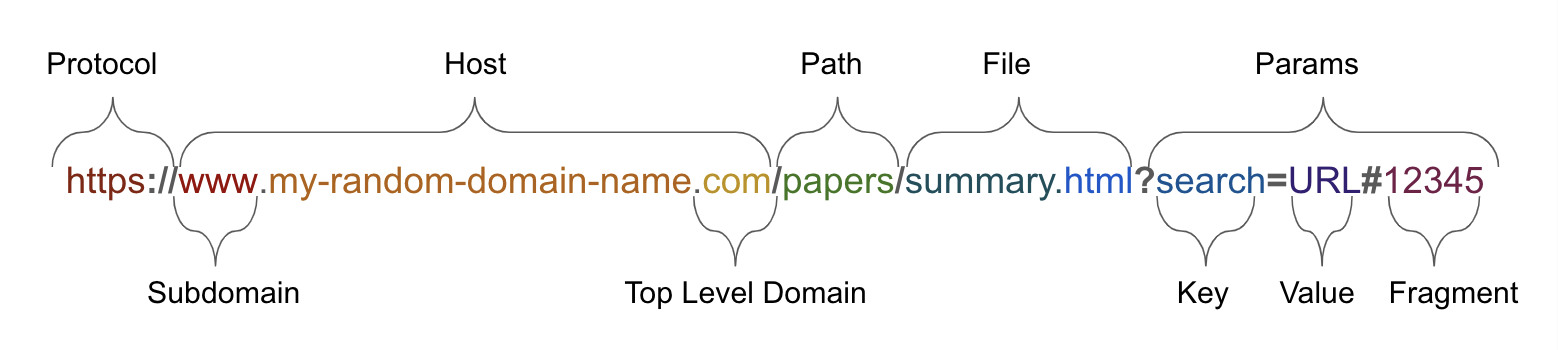
\includegraphics[scale=0.3]{images/URL_parts.png}
\caption{Structural components of a URL requiring specific feature engineering treatment}
\label{fig:url_structure}
\end{figure*}



\section{Methodology}

We design a feature extraction library for URLs that is sensitive to the various sections of URL
structure outlined above. We then apply this library to multiple machine learning tasks using only URLs
as the input variable. We experiment with multiple standard machine learning techniques and evaluate
the impact of the URL features using the SHAP package for feature importance.

\subsection{Features}

The features generated by the url2feature package are summairized in Table \ref{tab:features}

\begin{table*}
\caption{URL Features}
\label{tab:features}
\begin{tabular}{|l|l|l|l|}
\toprule
Group         &Feature              &Type        &Definition  \\
\midrule
Protocol      &protocol\_name         &Category    &The exact internet protocol name    \\
              &protocol\_type         &Category    &Internet protocol categorised by its purpose    \\
              &protocol\_exists       &Boolean     &Flag indicating presence or absence of internet protocol   \\
\midrule
Host          &host\_is\_ip           &Boolean     &Flag indicating if the host is an IP address    \\
              &host\_has\_port        &Boolean     &Flag indicating if a port number is explicitly specified    \\
              &domain\_sections       &Numeric     &Count of period separated domain sections    \\
              &domain\_reg\_year      &Numeric     &Year in which the domain was initially registered    \\
              &subdomain\_type        &Category    &Categorisation of the purpose of the subdomain \\
              &subdomain\_freq        &Numeric     &Frequency of the subdomain in internet traffics    \\
              &tld\_type              &Category    &Top Level Domain extension categorised by purpose    \\
              &tld\_freq              &Boolean     &Top Level Domain extension frequency in internet traffic   \\
\midrule
Path          &path\_depth            &Numeric     &The depth of the directory path between host and file   \\
              &path\_words            &Numeric     &Count of distinct words in the path between host and file   \\
              &path\_has\_date         &Boolean     &Flag indicating if a date is detected in the path  \\
              &path\_is\_home          &Boolean     &Flag indicating if the path starts with a home directory    \\
\midrule 
File          &file\_ext              &Category    &The exact file extension e.g. "exe" or "php"    \\
              &file\_type             &Category    &File extension categorised by function \& purpose    \\
              &file\_ext\_exists      &Boolean     &Flag indicating presence of a file extension for the URL target  \\
\midrule
Params        &params\_len            &Numeric     &The character length of the parameter string    \\
              &params\_count          &Numeric     &The count of the key value pairs in the param string    \\
              &params\_has\_url       &Boolean     &Flag indicating presence of a raw URL within the parameter string   \\
              &params\_enc\_url       &Boolean     &Flag indicating presence of an encoded URL within the parameter string   \\
              &params\_enc\_char      &Boolean     &Flag indicating presence of an encoded character within the parameter string   \\
              &params\_frag\_len      &Numeric     &Length of a hash delineated fragement at the end of the parameter string   \\
\bottomrule
\end{tabular}
\end{table*}



These URL feature functions are all available in the open source python package \emph{url2features}
available at https://pypi.org/project/url2features with links to usage documentation and source
code.

\subsection{Data}

The data used in this study was collected from a collction of publications that 
present internet classification problems containing URLs as the primary feature.
The ISCX Malcious URL classification dataset contains both malware and phishing URLS 
that need to be discriminated against benign URLS\cite{Mamun2016}.
The world wide web knowledge base (WebKb) 4 Universities data set contains a wide
range of university URLs categorised into multiple topic categories\cite{Craven1998}.
These 3 URL classification problems are summarised in Table \ref{tab:data}

The Syskill \& Webert webpage ratings dataset containing webepages across 4 categories
with \cite{Pazzani1996}

\begin{table}
\caption{Datasets}
\label{tab:data}
\begin{tabular}{|l|r|r|r|}
\toprule
Dataset              &Records        &Classes  &Majority    \\
\midrule
Malware              &46,944          &2       &            \\
Phishing             &45,343          &2       &            \\
WebKb 4Uni           &8,284           &7       &            \\
DMOZ                 &8,284           &7       &            \\
Syskill \& Webert     &8,284           &7       &            \\
\bottomrule
\end{tabular}
\end{table}

We generate all url features for each of these datasets and then apply a range of machine learning
techniques to build an appropriate classifier. 

\subsection{Feature Importance}

\begin{equation}
\label{campaign_baseline}
{}^c\mathcal{A}_p =  \frac{ \sum_{i \in I_p} \mathbf{1}^c(i) A_i }{ \sum_{i \in I_p} \mathbf{1}^c(i) }
\end{equation}


\section{Results}


\section{Conclusion}

\section{Acknowledgments}

\bibliographystyle{ACM-Reference-Format}
\bibliography{refs}

\end{document}
\endinput
%%
%% End of file `sample-sigconf.tex'.
